\documentclass[xcolor=table]{beamer}

% Inputs required
\usepackage{tikz}
\usepackage{svg}
\usepackage{color}
\usepackage{adjustbox}
\usetikzlibrary{timeline}

% Settings for the presentation
\usetheme{Hannover}
\setbeamerfont{footnote}{size=\tiny}
\setbeamerfont{subsection in toc}{size=\tiny}

% Title information
\title{Blockchain-based Payment for Carbon Trading}
\author[Oscar Golding]
{\textbf{Oscar Golding (z5160173)
\texorpdfstring{\\} 
\footnotesize Supervised by: Dr.~Sherry Xu, Dr.~Qinghua Lu}} 
\institute[UNSW]{Thesis B: UNSW}
\date{\today}

\begin{document}

% The title page
\begin{frame}
    \titlepage
\end{frame}

% The outline for the presentation
\begin{frame}{Outline}
    \tableofcontents
\end{frame}

% Sections to cover in the report
\section{Recap}
\subsection{Project Goals}
\begin{frame}{Problem}
    \begin{itemize}
        \item Energy production can be certified on the blockchain.
        \item Blockchain solves an Environmental,
              Social and Corporate Governance (ESG)
              problem for energy certification.
        \item Carbon trading is a politically contentious field lacking trust.
    \end{itemize}
\end{frame}
\begin{frame}{Aim}
    \begin{itemize}
        \item Can automated certification
              on the blockchain be used to deliver \textit{trust} in the market
              for carbon?
        \item Can blockchain-based hydrogen certification be used as a motivating
              example for carbon trading?
    \end{itemize}
\end{frame}
\begin{frame}{Thesis B Aims}
    \begin{itemize}
        \item Explore how \textit{Hyperledger Fabric} can be used to develop
              a blockchain carbon market.
        \item Understand the performance trade-offs
              of putting a carbon trading platform
              on the blockchain.
        \item Identify how ESG hydrogen certificates can be used to automate
              a carbon market.
    \end{itemize}
\end{frame}

\section{Blockchain Architecture}
\subsection{Overview}
\begin{frame}{Quick Overview}
    \begin{itemize}
        \item \textit{Hyperledger Fabric}
        \item Full stack blockchain application.
        \item User roles tied to a blockchain
              certificate authority - \textit{X.509} certificates.
        \item On-chain \textit{CouchDB} for indexed blockchain queries.
        \item Distributed smart contracts.
    \end{itemize}
\end{frame}
\subsection{User Roles}
\begin{frame}{User Roles}
    \begin{itemize}
        \item Energy producers and certifiers are registered with the
              Hyperledger Fabric Certificate Authority (CA).
        \item Upon account registration, a producer is registered with the CA.
        \item Chaincode is called on behalf of a producer/certifier.
        \item Distributed smart contracts for account creation.
    \end{itemize}
\end{frame}
\begin{frame}{Producer Creation Example}
    \begin{adjustbox}{max totalsize={1\textwidth}{0.85\textheight},center}
        \includesvg[inkscapelatex=false]{photos/AccountCreation.svg}
    \end{adjustbox}
\end{frame}
\subsection{Carbon Sales}
\begin{frame}{Carbon Sales}
    \begin{itemize}
        \item A producer is allowed to sell a fungible token called
              \textit{Carboncoin}.
        \item Offer for sale of tokens is stored on the blockchain.
        \item Aim is to encourage distributed trading of carbon using the
              blockchain as an intermediary.
        \item The producer entirely drives the trading process.
    \end{itemize}
\end{frame}
\begin{frame}{Carboncoin Sale Example}
    \begin{adjustbox}{max totalsize={1\textwidth}{0.85\textheight},center}
        \includesvg[inkscapelatex=false]{photos/CreateSale.svg}
    \end{adjustbox}
\end{frame}
\begin{frame}{Viewing Offers}
    \begin{itemize}
        \item An on-chain \textit{CouchDB} index is warmed for retrieving offers.
              \begin{itemize}
                  \item Warming happens whenever a new block is cut.
              \end{itemize}
        \item Optional \textit{carbon reputation} is attached to an offer
              so producers can ethically purchase carbon.
        \item Carbon reputation assists with increasing market quality.
    \end{itemize}
\end{frame}
\begin{frame}{Retrieving Offers Example}
    \begin{adjustbox}{max totalsize={1\textwidth}{0.85\textheight},center}
        \includesvg[inkscapelatex=false]{photos/GetOffersNo.svg}
    \end{adjustbox}
\end{frame}
\subsection{Direct Market Interaction}
\begin{frame}{Direct Market Interaction}
    \begin{itemize}
        \item A producer can directly purchase
              \textit{Carboncoin} outside of the open market
              at an \textit{extra cost}.
        \item The user is given an on-chain offer token to purchase
              \textit{Carboncoin}.
        \item The price per token is calculated using the maximum offer on the
              open market.
        \item Each $x_i$ in Equation~\ref{eq:1} represents an active offer
              in the market.
    \end{itemize}
    \begin{equation}
        \text{Direct Offer} =
        \max \left(\left\langle x_1, x_2, \dots, x_n \right\rangle\right) + 50
        \label{eq:1}
    \end{equation}
\end{frame}
\begin{frame}{Direct Offer Creation Example}
    \begin{adjustbox}{max totalsize={1\textwidth}{0.85\textheight},center}
        \includesvg[inkscapelatex=false]{photos/directOffer.svg}
    \end{adjustbox}
\end{frame}
\subsection{ESG Certificates}
\begin{frame}{ESG Certificate Interaction}
    \begin{itemize}
        \item Market activity triggered by an ESG certifier recording
              carbon production.
        \item As a step in certificate creation, the certifier invokes
              the carbon market smart contract.
        \item Both the certifier and the carbon market exist on the
              same \textit{Hyperledger} channel.
        \item If the user does not have enough \textit{Carboncoin}
              to pay for production, then a debt is recorded.
    \end{itemize}
    \begin{figure}
        \caption{Channel Interaction}
        \centering
        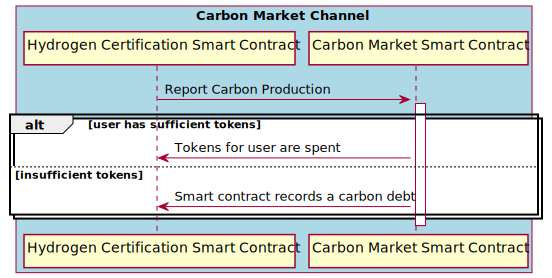
\includegraphics[height=0.5\textheight, width=0.5\linewidth,
            keepaspectratio]{photos/chain.png}
    \end{figure}
\end{frame}


\section{Blockchain Patterns}
\subsection{Patterns Overview}
\begin{frame}{Patterns}
    \begin{itemize}
        \item Token template
        \item Policy contract
        \item Token registery
        \item Token swap
        \item Burned token
    \end{itemize}
    \begin{figure}
        \caption{Carboncoin Lifecycle}
        \centering
        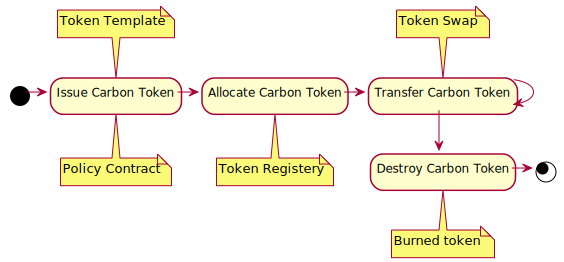
\includegraphics[height=0.5\textheight, width=0.6\linewidth,
            keepaspectratio]{photos/Token.png}
    \end{figure}
\end{frame}
\subsection{Policy Contract}
\begin{frame}{Policy Contract Pattern}
    \begin{itemize}
        \item All blockchain operations are bounded by policies which
              provide rules on how \textit{Carboncoin} can be used.
        \item Only producers with the \textit{producer} role can buy or
              sell \textit{Carboncoin}.
        \item A user can never sell more \textit{Carboncoin} than the amount
              contained inside their account.
        \item A user's \textit{X.509} certificate is required to perform write
              operations on the blockchain.
    \end{itemize}
\end{frame}
\subsection{Token Swap}
\begin{frame}{Token Swap Pattern}
    \begin{itemize}
        \item \textit{Carboncoin} can be swapped between users.
        \item Policies are attached when doing a swap:
              \begin{itemize}
                  \item Active offer is required.
                  \item Seller must have enough \textit{Carboncoin}.
                  \item The buyer must meet their open offer obligations first
                        before purchasing tokens.
              \end{itemize}
        \item The swap happens for only the \textit{Carboncoin} token.
    \end{itemize}
\end{frame}
\subsection{Burned Token}
\begin{frame}{Burned Token}
    \begin{itemize}
        \item A \textit{Carboncoin} is burned when a producer is required
              to pay for carbon production.
        \item \textit{Digital Physical Parity} exists between real carbon
              production and the carbon reputation in the market.
              \begin{itemize}
                  \item Certifiers play a signficant role in maintaining the
                        digital physical parity between carbon production and
                        carbon reputation.
              \end{itemize}
        \item Debts are recorded when a user does not have enough
              \textit{Carboncoin} to pay for carbon production. Debts can
              be paid at later dates.
    \end{itemize}
\end{frame}

\section{Blockchain Performance}
\begin{frame}{System Performance}
    \begin{itemize}
        \item Although the aim of the thesis is not to produce the most
              high throughput carbon market - the performance of the
              system is still worth exploring.
        \item The performance of \textit{Fabric} has a tendency to
              suffer in the \textit{Validation Phase} of the transaction lifecycle.
        \item An observed tendency of Hyperledger is that as the transactions
              per second (TPS) increases, so do
              errors~\cite{10.1145/3448016.3452823}.
    \end{itemize}
\end{frame}
\subsection{Bottlenecks}
\begin{frame}{Common Bottlenecks}
    \begin{itemize}
        \item Multi-Version Concurrency Control (MVCC) - transactions in the
              same block updating the same key (transaction dependency).
        \item Phantom Read Conflicts - performing a read on a key range
              which has been updated.
              \begin{itemize}
                  \item For some reading range $i$ to $j$,
                        if a key has recently
                        been inserted then read a phantom read happens.
              \end{itemize}
    \end{itemize}
\end{frame}
\subsection{TPS Enhancements}
\begin{frame}{Enhancements to TPS}
    \begin{itemize}
        \item Represent assets on the blockchain as a sum of deltas to avoid
              MVCC errors.
        \item Example: CarbonCoin is the sum of deltas in Equation~\ref{eq:2}.
              \begin{itemize}
                  \item Each $\delta_i$ contains a unique combination of owner,
                        transaction identifier and sign.
                  \item Each $x_i$ represents the asset value (for example 500).
              \end{itemize}
        \item Localise the phantom read conflicts into `low TPS' domains.
    \end{itemize}
    \begin{equation}
        \text{Asset Value} = \delta_1 x_1 + \delta_2 x_2 + \dots + \delta_n x_n
        \label{eq:2}
    \end{equation}
\end{frame}

\section{Thesis B Plan}
\begin{frame}{Original Research Timeline}
    \begin{adjustbox}{max totalsize={.9\textwidth}{.7\textheight},center}
        \begin{tikzpicture}[timespan={}]

            \timeline[custom interval=true]{Thesis A, Thesis B, Thesis C}

            % Phases for the project
            \begin{phases}
                \initialphase{involvement degree=1.75cm,phase color=black}
                \phase{between week=1 and 3 in 0.01,involvement degree=2cm}
                \phase{between week=1 and 2 in 0.4,involvement degree=3cm}
                \phase{between week=1 and 2 in 1.1,involvement degree=5cm}
                \phase{between week=2 and 3 in 1.1, involvement degree=6cm}
            \end{phases}

            % Project milestones 0-360 on the individual phase
            \addmilestone{at=phase-0.90,direction=90:1cm,
                text={Initial meeting},
                text options={above}}
            \addmilestone{at=phase-0.270,direction=270:1cm,
                text={Blockchain Patterns},text options={below}}
            \addmilestone{at=phase-1.240,direction=240:1cm,
                text={Domain Analysis},text options={below}}
            \addmilestone{at=phase-2.110,direction=120:1.5cm,
                text={Investigate Technical Details},text options={above}}
            \addmilestone{at=phase-2.250,direction=240:1.5cm,
                text={Literature Review},text options={below}}
            \addmilestone{at=phase-3.250,direction=240:1.5cm,
                text={Create Architecture},text options={below}}
            \addmilestone{at=phase-4.250,direction=240:1.5cm,
                text={Create User Interface},text options={below}}
            \addmilestone{at=phase-3.75,direction=120:1.5cm,
                text={Develop Chaincode},text options={above}}
            \addmilestone{at=phase-4.0035,direction=45:2.5cm,
                text={Improvements},text options={above}}
            \addmilestone{at=phase-4.125,direction=45:2.5cm,
                text={Chain Authorities},text options={above}}
        \end{tikzpicture}
    \end{adjustbox}
\end{frame}
\begin{frame}{Updated Research Timeline}
    \begin{adjustbox}{max totalsize={.9\textwidth}{.7\textheight},center}
        \begin{tikzpicture}[timespan={}]

            \timeline[custom interval=true]{Thesis A, Thesis B, Thesis C}

            % Phases for the project
            \begin{phases}
                \initialphase{involvement degree=1.75cm,phase color=black}
                \phase{between week=1 and 3 in 0.01,involvement degree=2cm}
                \phase{between week=1 and 2 in 0.4,involvement degree=3cm}
                \phase{between week=1 and 2 in 1.1,involvement degree=5cm}
                \phase{between week=2 and 3 in 1.1, involvement degree=6cm}
            \end{phases}

            % Project milestones 0-360 on the individual phase
            \addmilestone{at=phase-0.90,direction=90:1cm,
                text={Initial meeting},
                text options={above}}
            \addmilestone{at=phase-0.270,direction=270:1cm,
                text={Blockchain Patterns},text options={below}}
            \addmilestone{at=phase-1.240,direction=240:1cm,
                text={Domain Analysis},text options={below}}
            \addmilestone{at=phase-2.110,direction=120:1.5cm,
                text={Investigate Technical Details},text options={above}}
            \addmilestone{at=phase-2.250,direction=240:1.5cm,
                text={Literature Review},text options={below}}
            \addmilestone{at=phase-3.250,direction=240:1.5cm,
                text={Create Architecture},text options={below}}
            \addmilestone{at=phase-3.275,direction=290:2.0cm,
                text={Create User Interface},text options={below}}
            \addmilestone{at=phase-3.120,direction=120:1.5cm,
                text={Develop Chaincode},text options={above}}
            \addmilestone{at=phase-4.090,direction=45:2.5cm,
                text={Improvements},text options={above}}
            \addmilestone{at=phase-3.090,direction=45:2.5cm,
                text={Chain Authorities},text options={above}}
        \end{tikzpicture}
    \end{adjustbox}
\end{frame}
\begin{frame}{Table Representation}
    \begin{itemize}
        \item Original plan for Thesis B. Green records the task being completed.
    \end{itemize}
    \begin{table}[]
        \caption{Plan for Thesis B}
        \label{tab:my-table}
        \begin{tabular}{|l|l|}
            \hline
            Week & Plan                                                                   \\ \hline
            1    & \cellcolor[HTML]{32CB00}Hyperledger Documentation                      \\ \hline
            2    & \cellcolor[HTML]{32CB00}Hyperledger Documentation                      \\ \hline
            3    & \cellcolor[HTML]{32CB00}Hyperledger Documentation                      \\ \hline
            4    & \cellcolor[HTML]{32CB00}Smart Contract Programming - Producer Register \\ \hline
            5    & \cellcolor[HTML]{32CB00}Smart Contract Programming - Offer Lifecycle   \\ \hline
            6    & \cellcolor[HTML]{32CB00}Smart Contract Programming - Carbon Reputation \\ \hline
            7    & \cellcolor[HTML]{32CB00}Smart Contract Programming - Direct Purchase   \\ \hline
            8    & \cellcolor[HTML]{32CB00}API Construction - Account Creation            \\ \hline
            9    & \cellcolor[HTML]{32CB00}API Construction - Wiring Requests to Offers   \\ \hline
            10   & \cellcolor[HTML]{32CB00}API Construction - UI Functionality            \\ \hline
        \end{tabular}
    \end{table}
\end{frame}
\begin{frame}{Plan Update}
    \begin{itemize}
        \item Ahead of schedule - working prototype with chaincode, implemented
              architecture and a user interface.
        \item Plan for Thesis C:
              \begin{itemize}
                  \item Exploration of blockchain performance (TPS).
                  \item Generalisation of blockchain patterns to sources of
                        energy outside of hydrogen - for example water.
                  \item The auctioning of \textit{Carboncoin} to hydrogen
                        producers.
                  \item Payment channel for recording off-chain transactions.
              \end{itemize}
    \end{itemize}
\end{frame}

\section{References}
\begin{frame}[allowframebreaks]{References}
    \bibliographystyle{plain}
    \nocite{*}
    {\footnotesize
        \bibliography{ass}}
\end{frame}

\end{document}
